%%This is a very basic article template.
%%There is just one section and two subsections.
\documentclass[11pt, a4paper, reqno, twoside]{scrartcl}

\usepackage[a4paper, hmargin={1in, 1in}, vmargin={1in,
  1in},headsep=10mm,headheight=5mm,footskip=30pt]{geometry}
 \usepackage{graphicx}
\usepackage{epsfig}
\usepackage{epstopdf}
\graphicspath{ {./images/} }

\usepackage{ amsmath, amssymb,amsthm}
\usepackage{hyperref}
\usepackage{bm,color}
\usepackage{verbatim}
\usepackage{wrapfig}
\usepackage{caption}
\usepackage{subcaption}
\usepackage{tikz}
\usepackage{tkz-euclide}
\usetkzobj{all}
\usepackage[boxruled,commentsnumbered]{algorithm2e}
\usepackage{booktabs}

\usepackage{fancyhdr}
  \renewcommand{\baselinestretch}{0.97} %this factor controls the space between lines
  \fancyhead[]{}
  \renewcommand{\headrulewidth}{0pt}

% the only way to get two column algorithms seems to be to use a hack on top of the algorithm2e package
\usepackage{multicol}
%\usepackage[ruled,commentsnumbered]{algorithm2e}

\newenvironment{algo}{%
  \renewenvironment{algocf}[1][h]{}{}% pass over the floating stuff
  \algorithm
}{%z
  \endalgorithm
}

\definecolor{darkgreen}{rgb}{0,.4,.2}
\definecolor{darkblue}{rgb}{.1,.2,.6}
\definecolor{brightblue}{rgb}{0,0.6,0.8}
\hypersetup{
  colorlinks=true,
  linkcolor=darkblue,
  citecolor=darkgreen,
  filecolor=darkblue,
  urlcolor=darkblue
}
\usepackage{pifont}% http://ctan.org/pkg/pifont
\newcommand{\cmark}{\ding{51}}%
\newcommand{\xmark}{\ding{55}}%

\addtokomafont{caption}{\small}
\addtokomafont{captionlabel}{\sffamily\bfseries}

\newtheoremstyle{style}
 {\topsep}              % Space above
 {\topsep}              % Space below
 {\itshape}              % Body font: original {\normalfont}
 {}                         % Indent amount (empty = no indent,%\parindent = paraindent)
 {\sffamily\bfseries}  % Thm head font original
 {.}	                     % Punctuation after thm head
 { }                         % Space after thm head (\newline = linebreak)
 {}                          % Thm head spec
\theoremstyle{style}

%%%%%%%%%%%%%%%%%%%%%%%%%%%%%%%%%%%%%%%%%%%
%%% Environments, Definitions, Commands %%%
%%%%%%%%%%%%%%%%%%%%%%%%%%%%%%%%%%%%%%%%%%%

\newtheorem{definition}{Definition}
\newtheorem{theorem}{Theorem}
\newtheorem{proposition}[definition]{Proposition}
\newtheorem{lemma}{Lemma}
\newtheorem{corollary}[definition]{Corollary}
\newtheorem{observation}[definition]{Observation}
\newtheorem{conjecture}[definition]{Conjecture}
\newtheorem{remark}[definition]{Remark}
\newtheorem{problem}{Problem}
\newtheorem{claim}{Claim}
\newtheorem{open}{Open Problem}
\newtheorem*{example}{Example}

% the * at the end of operator seems to have the effect that the command will be properly have its sub/superstripts vertically below/above it, like \sum for example, this only applies if you are in \displaystyle
\DeclareMathOperator{\st}{\textrm{s.t.}}
\DeclareMathOperator*{\conv}{conv}
\DeclareMathOperator{\diam}{diam}
\DeclareMathOperator*{\E}{\rm E}
\DeclareMathOperator*{\argmin}{\arg\min}
\DeclareMathOperator*{\argmax}{\arg\max}
\DeclareMathOperator{\lmax}{\lambda_{\max}}
\DeclareMathOperator{\lmin}{\lambda_{\min}}
\DeclareMathOperator*{\supp}{supp}
\DeclareMathOperator*{\diag}{diag}
\DeclareMathOperator*{\sign}{sign}
\DeclareMathOperator*{\tr}{Tr}
\DeclareMathOperator*{\rk}{Rk}
\DeclareMathOperator*{\card}{card}
\DeclareMathOperator*{\nnz}{nnz}
\DeclareMathOperator*{\relint}{\mathop{relint}}

%norms
\providecommand{\abs}[1]{\left\lvert#1\right\rvert}
\providecommand{\norm}[1]{\left\lVert#1\right\rVert}

\newcommand{\ball}{\mathcal{B}}
\newcommand{\sphere}{\mathcal{S}}

\newcommand{\bigO}{O}
\newcommand{\R}{\mathbb{R}}
\newcommand{\X}{\mathcal{X}}
\newcommand{\Sym}{\mathcal{S}}
\newcommand{\Supt}{\Sym_{(t)}}
\newcommand{\Suptc}{\bar{\Sym}_{(t)}}

\newcommand{\appcof}{v}
\newcommand{\domain}{\mathcal{D}}

\newcommand{\points}{\mathcal{A}}
\newcommand{\stepsize}{\gamma}
\newcommand{\Cf}{C_{\hspace{-0.08em}f}}
\newcommand{\x}{\bm{x}}
\newcommand{\y}{\bm{y}}
\newcommand{\z}{\bm{z}}
\newcommand{\s}{\bm{s}}
\newcommand{\shat}{\bm{\hat{s}}}
\newcommand{\bv}{\bm{b}}
\newcommand{\dv}{\bm{d}}
\newcommand{\qv}{\bm{q}}
\newcommand{\uv}{\bm{u}}
\newcommand{\av}{\bm{v}}
\newcommand{\vv}{\bm{v}}
\newcommand{\wv}{\bm{w}}
\newcommand{\xv}{\bm{x}}
\newcommand{\row}{\text{row}}
\newcommand{\col}{\text{col}}
\newcommand{\lft}{\text{left}}
\newcommand{\rgt}{\text{right}}
\newcommand{\dualp}{\bm{\alpha}}
\newcommand{\indic}{\mathbb{I}}
%
\newcommand{\signVec}{\mathbf{s}}
\newcommand{\N}{\mathbb{N}}
\newcommand{\F}{\mathbb{F}}
\newcommand{\M}{\mathbb{M}}
\newcommand{\id}{\mathbf{I}} % big i for identity
\newcommand{\ind}{\mathbf{1}} % indicator vectors
\newcommand{\0}{\mathbf{0}} % the origin
\newcommand{\unit}{\mathbf{e}} % unit basis vectors
\newcommand{\one}{\mathbf{1}} % all one vector
\newcommand{\zero}{\mathbf{0}}
\newcommand\SetOf[2]{\left\{#1\vphantom{#2}\right.\left|\vphantom{#1}\,#2\right\}}
\newcommand{\ignore}[1]{}%{\textbf{***begin ignore***}\\#1\textbf{***end ignore***}}


\newcommand{\todo}[1]{\marginpar[\hspace*{4.5em}\textbf{TODO}\hspace*{-4.5em}]{\textbf{TODO}}\textbf{TODO:} #1}
\newcommand{\idea}[1]{\marginpar[\hspace*{4.5em}\textbf{IDEA}\hspace*{-4.5em}]{\textbf{IDEA}}\textbf{IDEA:}
#1}
\newcommand{\note}[1]{\marginpar{#1}}





\begin{document}
\pagestyle{fancy}



%%%%%%%%%%%%%%%%%%%%%%%%%%%%%%%%
\title{Importance Sampling Using LSH: A novel variance reduction method}

%\author{\\ Author Name\\
%{\small \href{mailto:author@ethz.ch}{author@ethz.ch}}}
\date{} 

\maketitle


\textbf{Introduction:}
Given an objective function on the sum of training samples points $\x_i$, we
want to compute the minimiser of this convex objective function using SGD; 
\begin{equation*}
	\wv^*_n = \arg \min_{\wv} \bigg[ \sum_{i=1}^n \phi(\x_i;\wv) = \sum_{i=1}^n
	\phi_i(\wv) \bigg]
\end{equation*}
 The idea is based on the paper \cite{zhao2014stochastic}, where the
 authors found the perfect importance sampling for variance reduction of SGD
 [equation 5]; More preciously, they proved if we want to reduce the variance
 of SGD the most, the best sampling approach is sampling according to the norm
 of stochastic gradient elements, i.e. :
\begin{equation*}
	p(\x_i) = \frac{\|\nabla \phi_i(\wv^t)\|_2}{\sum_i \|\nabla \phi_i(\wv^t)\|_2}
\end{equation*}
The authors mentioned we have to compute the gradient respect to all training
points $\x_i$, then they provide an importance sampling which is completely
independent of current estimated parameters $\wv^t$. We want to do sampling without
computing all gradients that depends on the current estimated parameter $\wv^t$;
But how we can do this? Consider the least squared problem for which the loss is $\phi(\x_i;\wv) = (\langle \x_i, \wv \rangle -
y_i)^2 $ and its gradient is $\nabla \phi_i(\wv) = 2 x_i^T(\langle \x_i, \wv \rangle -
y_i)$. Assume all the training points $\x_i$ are normalized; In this case, the
norm is $\|\nabla \phi_i(\wv)\| = 2 |\langle \x_i, \wv \rangle -
y_i|$. We can define new vectors $\z_i = [\x_i,y_i]$ and $\qv = [\wv,-1]$ and
rewrite the norm of gradient as: 
\begin{equation*}
	\nabla \phi_i(\wv) = 2 |\langle \z_i, \qv \rangle| = 2 \|\z_i\| \|\qv\|
	|\cos[\angle(\z_i,\qv)]|
\end{equation*}
Since all data points $\xv_i$ are normalized, we can assume the 
$\|\z_i\|$ are almost normalized as well and just focus on the cosine term. 
Here, the local sensitive hash function comes to picture; 
Let's recap what the a simple local sensitive hash function does; Consider we
pick a random Gaussian vector $\uv$ and design a hash function thereby in the
following way:
\begin{equation*}
	h_{\uv}(\z) = \text{sign(} \langle \uv, \z \rangle \text{)}
\end{equation*}
Then, we can easily prove this simple hashing function is a good angular sampler
means \cite{charikar2002similarity}:
\begin{equation*}
	P[h_{\uv}(\z_i) = h_{\uv}(\qv)] = 1-\frac{\angle(\z_i,\qv)}{\pi}.
\end{equation*}
Now, the question is how we can use a set of this angular sampler to design a
local sensitive hashing function that provide us cosine sampler; 
\begin{equation*}
	P[Z_i = 1] \sim \frac{|\cos(\angle(\z_i,\qv))|}{\sum_{j}
	|\cos(\angle(\z_j,\qv))|},
\end{equation*}
where the $Z_i$ is a binary random variable that is a compact notation for
hashing function depends on $\qv$ and $\z_i$.
\begin{equation*}
	Z_i = \indic[h(\z_i) = h(\qv)]
\end{equation*}
 For simplicity we use the relaxed
absolute values of cosines:
\begin{equation*}
 P[Z_i] \sim \frac{\cos^2(\angle(\z_i,\qv))}{\sum_{j}
	\cos^2(\angle(\z_j,\qv))}
\end{equation*}
\textbf{Motivational Experiment:}
Our experiments show that cosine sampler improves the convergence of SGD
considerably (Figure \ref{fig:convergence_cosine_sampler}). In this experiment
we use least squared objective function without any regularizer with normalized
training points. \\
\textbf{More Discussions:} 
Consider the new notation $\theta_i = \angle(\z_i,\qv)$. 
If we were given a local sensitive hash function for squared cosine similarity,
i.e. $\cos^2(\theta_i)$, then we could easily design a $\cos^2$-sampler. The
definition of LSH for squared cosine similarity is a hash function $h$ with
stochastic binary output $Z_i = \indic[h(\z_i) = h(\qv)]$ with the probability
proportional to  $\cos^2(\theta_i)$. 
\begin{equation*}
	P[Z_i = 1] = \cos^2(\theta_i) 
\end{equation*}
Using above LSH, we can design the a new hash function for $\sum_i
\cos^2(\theta_i)$ as:
\begin{eqnarray*}
	& \E [\sum_i Z_i] & = \sum_i \E [Z_i]\\
	& & = \sum_i P[Z_i = 1] = \sum_i\cos^2(\theta_i)
\end{eqnarray*} 
Therefore, if we uniformly return a random point which has the same hash value
as the hash value of the query, i.e. $h(\z_i) = h(\qv)$, then $P[h(\z_i) =
h(\qv)] = \frac{\cos^2 \theta_i}{\sum_i \cos^2(\theta_i)}$.
Now, hashing with probability respect to the $\cos^2(\theta_i)$ remains.
Our initial idea is using infinite product decomposition of cosine function:
\begin{eqnarray*}
	& \cos(\theta_i) & = \prod_{n=1}^{\infty} \bigg[1-\frac{4
	\theta_i^2}{\pi^2(2n-1)^2}\bigg] \\
	& & \simeq \bigg[1-\frac{4
	\theta_i^2}{\pi^2}\bigg] \bigg[ 1-\frac{\theta_i^2}{9/4 \pi^2} \bigg]
\end{eqnarray*}
The general form of these products is $1-\alpha \frac{\theta^2_i}{\pi^2} $; Now
we suggest a hashing function which give us the $1-\frac{\theta^2}{\pi^2}$.
We pick two \textbf{independent} random vectors $\uv$ and $\vv$, then following
hashing technique give us the probability $1-\frac{\theta^2}{\pi^2}$: 
\begin{eqnarray*}
	& P\bigg[  h_{\uv}(\z_i) = h_{\uv}(\qv) \vee h_{\vv}(\z_i) = h_{\vv}(\qv)
	\bigg] & = 1 - P\bigg[  h_{\uv}(\z_i) \neq h_{\uv}(\qv) \wedge h_{\vv}(\z_i)
	\neq h_{\vv}(\qv) \bigg] \\
	& & = 1-\frac{\theta^2}{\pi^2}
\end{eqnarray*}
Still, we don't know how can we reconstruct a random variable with distribution 
$1-\frac{4
	\theta_i^2}{\pi^2}$. First of all, this value is not a valid distribution
	function which gets the negative values as well. So, the question is how
	can we reconstruct this function using a collection of random variables that
	all distributed as $\frac{\theta}{\pi}$. The boolean operator such as and, or, and
	not are our tools to reconstruct the cosine distribution. \\
\textbf{Future Plan:}
The squared cosine LSH paves our ways towards a better approximated inner
product search. The general issue of LSH for inner product (as well cosine
similarity) is estimating inner product using angular distance, which is very
crude. Our next step is using the cosine LSH to improve approximate maximum
inner product search.\\ 
Let's go back to our main goal that was sampling the points proportional to
their norm of stochastic gradient. Our past approach, using LSH, tried to
split all space to some blocks using random hyper-planes; The random
partitioning of whole space is quit inefficient. Can we cluster the data and using
the center of clusters to design an inner product sampler? 
 \begin{figure}
    \centering
        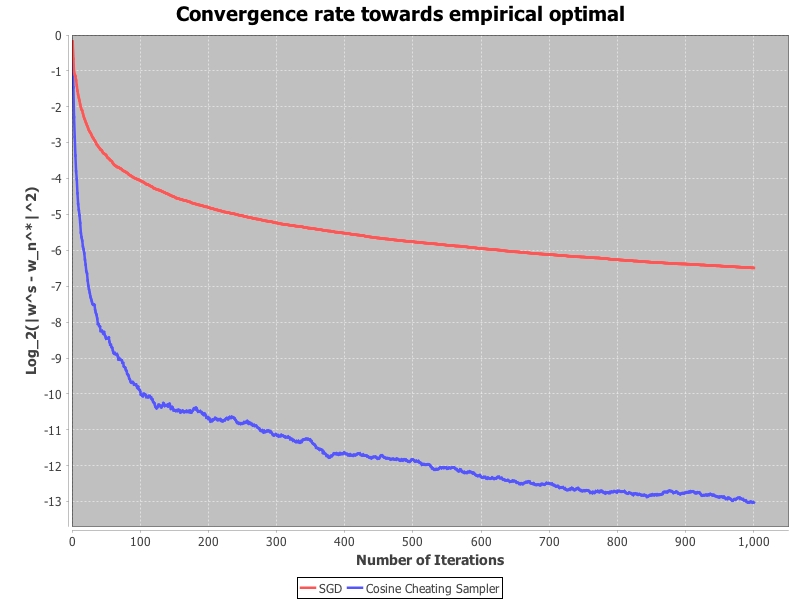
\includegraphics[width=0.8\textwidth]{empirical_importance_cosine.JPEG}
    \caption{The Perfect Cosine Sampler
    Performance}\label{fig:convergence_cosine_sampler}
 \end{figure}


\bibliographystyle{alpha}
\bibliography{bibliography}


\end{document}
